\chapter{OVERVIEW}
\label{Chapter2}

The gesture generation problem, like other machine learning tasks, has been studied and developed alongside both traditional and modern machine learning methods. These include rule-based and data-driven approaches. This thesis first presents the characteristics of gestures \autoref{sec:relationspeechandgesture}, serving as the foundation for learning the relationship between gestures, text, and speech. In section \autoref{sec:commonstage}, the thesis introduces the common stages across different gesture generation methods.

In section \autoref{sec:relatedwork}, the thesis presents the methods that have been applied in gesture generation. A comparison of these methods is provided, leading to the motivation for adopting diffusion models for this task.

Section \autoref{sec:diffusionbase} explains how diffusion models have recently been applied to gesture generation.

\section{Gesture Characteristics}
\label{sec:relationspeechandgesture}

According to linguistics, gestures can be categorized into six main groups: adaptors, emblems, deictics, iconics, metaphorics, and beats \cite{ekman1969repertoire}, \cite{sebeok2011advances}. Among them, beat gestures do not carry direct semantic meaning but play an important role in synchronizing rhythm between speech and gesture \cite{kipp2005gesture}, \cite{sebeok2011advances}. However, the rhythm between speech and beat gestures is not fully synchronized, making the temporal alignment between them complex to model \cite{mcclave1994gestural}, \cite{bhattacharya2021speech2affectivegestures}, \cite{kucherenko2020gesticulator}, \cite{yoon2020speech}.

Gestures interact with various levels of information in speech \cite{sebeok2011advances}. For instance, emblematic gestures like a thumbs-up are usually linked to high-level semantic content (e.g., “good” or “excellent”), while beat gestures often accompany low-level prosodic features such as emphasis. Previous studies typically extract features from the final layer of the speech encoder to synthesize gestures \cite{alexanderson2020style}, \cite{bhattacharya2021speech2affectivegestures}, \cite{kucherenko2021large}, \cite{qian2021speech}, \cite{yoon2022genea}. However, this approach may blend information from different levels, making it hard to disentangle rhythm and semantics.

As shown in linguistic studies \cite{kipp2005gesture}, \cite{neff2008gesture}, \cite{webb1997linguistic}, gestures in daily communication can be decomposed into a limited number of semantic units with various motion variations. Based on this assumption, speech features are divided into two types: high-level features representing semantic units and low-level features capturing motion variations. Their relationships are learned across different layers of the speech encoder. Experiments demonstrate that this mechanism can effectively disentangle features at different levels and generate gestures that are both semantically and stylistically appropriate.

\section{Overview of Gesture Generation Methods}
\label{sec:relatedwork}

\subsection{Rule-Based Methods}

\subsubsection{General Principle}

These methods rely on clearly defined rules, which are manually crafted to determine how the system processes inputs to produce outputs.

\subsubsection{Methods}

Representative rule-based methods include the \textit{Robot behavior toolkit} \cite{huang2012robot} and \textit{Animated conversation} \cite{cassell1994animated}. These approaches typically map speech to gesture units using handcrafted rules. Rule-based systems allow for straightforward control over model outputs and provide good interpretability.  
However, the cost of manually designing these rules is prohibitive for complex applications requiring the processing of large-scale data.

\subsection{Statistical Methods}

\subsubsection{General Principle}

These methods rely on data analysis, learning patterns from datasets, and using probabilistic models or mathematical functions for prediction. The approach involves optimizing model parameters to fit the data.

\subsubsection{Methods}

Like rule-based methods, data-driven methods also map speech features to corresponding gestures. However, instead of manual rules, they employ automatic learning based on statistical data analysis.

Representative statistical approaches include \textit{Gesture controllers} \cite{levine2010gesture}, \textit{Statistics-based} \cite{yang2020statistics}, which use probabilistic distributions to find similarities between speech and gesture features. \textit{Gesture modeling} \cite{neff2008gesture} constructs probabilistic models to learn individual speaker styles.

\subsection{Deep Learning Methods}

\textbf{General Principle of Deep Learning Methods}

These methods utilize multi-layer perceptrons (MLPs) to automatically extract features from raw data and learn complex data representations through parameter optimization.

\begin{figure}[H]
	\centering
	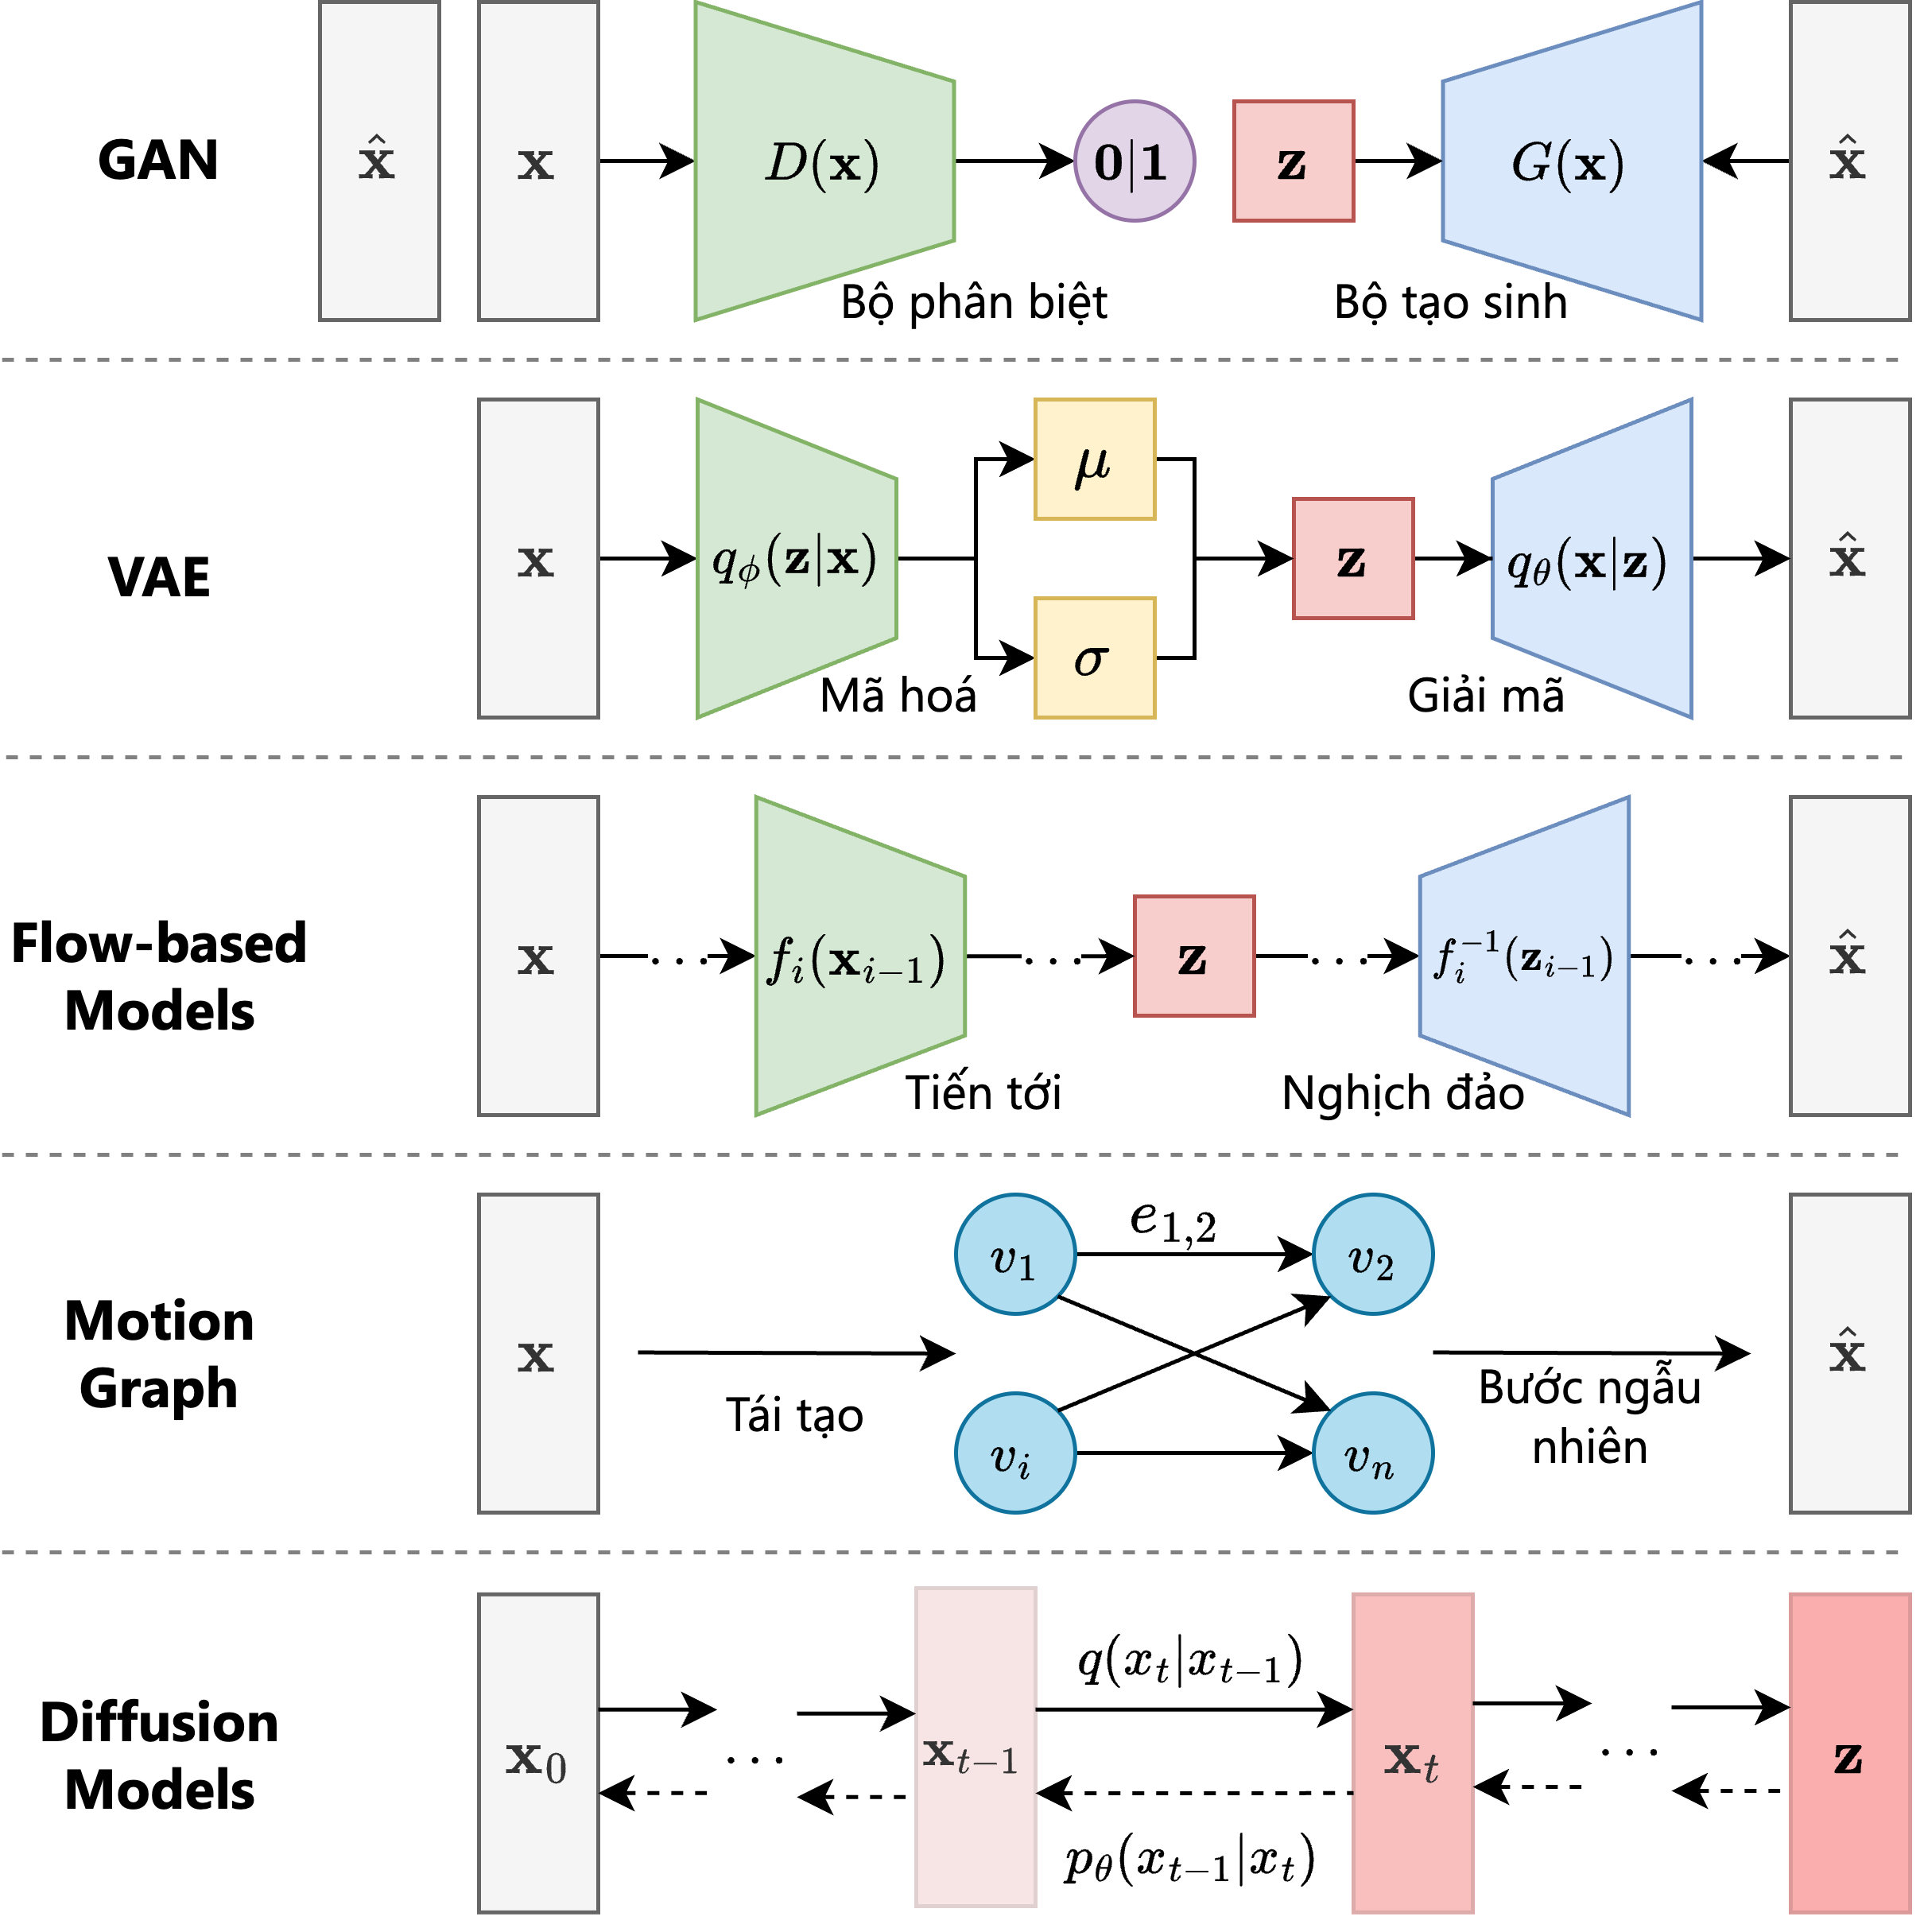
\includegraphics[width=0.8\textwidth]{GeneralOverview}
	\caption{Overview of different generative models.}
	\label{fig:GeneralOverview}
\end{figure}

As illustrated in \autoref{fig:GeneralOverview}, deep learning-based gesture generation methods can be divided into two main groups: likelihood-based models and implicit generative models \cite{song2021score}.

\subsubsection{Likelihood-Based Models}

\textbf{General Principle of Likelihood-Based Models}

These models work by maximizing the likelihood of observed data given model parameters $\theta$. The objective is to find the optimal parameters $\theta'$ by modeling the probability $p(\mathbf{x})$ of the data, where $\mathbf{x}$ represents the gesture sequence.

\textbf{Methods}

The application of deep learning to gesture generation has evolved alongside the development of deep learning models, including RNNs, LSTMs, and Transformers. Representative likelihood-based methods include:

\begin{itemize}[]
	\item \textit{Gesticulator} \cite{kucherenko2020gesticulator}, which uses a Multilayer Perceptron (MLP) to encode text and audio features, with BERT-derived vectors used as text features.

	\item \textit{HA2G} \cite{liu2022learning} builds a hierarchical Transformer-based model to learn multi-level correlations between speech and gestures, from local to global features.

	\item \textit{Gesture Generation from Trimodal Context} \cite{yoon2020speech} uses an RNN architecture and treats gesture generation as a translation task in natural language processing.

	\item \textit{DNN} \cite{chiu2015predicting} combines LSTM and GRU to build a classifier neural network that selects appropriate gesture units based on speech input.

	\item \textit{Cascaded Motion Network (CaMN)} \cite{liu2022beat} introduces the BEAT dataset and a waterfall-like model. Speaker information, emotion labels, text, speech, and gesture features are processed through layers to extract latent vectors. In the fusion stage, CaMN combines features sequentially: speaker and emotion features are merged first, followed by integration with latent vectors of text, speech, and gestures.

	\item \textbf{Motion Graph}: In \textit{Gesturemaster} \cite{zhou2022gesturemaster}, a semantic graph is constructed where words in a sentence are connected based on semantic relationships. The model then selects the most relevant nodes and edges in the graph to represent gestures.
\end{itemize}


\subsubsection{Implicit Generative Models}
\label{sec:ImplicitGenerativeModels}

\textbf{Principle}

Implicit generative models learn the data distribution without explicitly modeling the probability density function $p(\bx)$. Instead of directly computing $p(\bx)$, the model learns a mapping $G_{\theta}: \mathcal{Z} \to \mathcal{X}$ by matching the distributions between real and generated data $\mathbf{x} = G_\theta(\mathbf{z}), \quad \mathbf{z} \sim p_z(\mathbf{z})$. Here, $\mathcal{Z}$ denotes the input noise space, typically with a simple distribution \(p_{z}\) (e.g., Gaussian, Uniform), and \(\mathcal{X}\) is the space of real data, which in this case is gesture sequences \(\mathbf{x}\).

In gesture generation, to incorporate conditions such as speech or text labels, implicit generative models often introduce a condition $\mathbf{c}$ representing the context of the task, resulting in the conditional generation: $\mathbf{x} = G_\theta(\mathbf{z}, \mathbf{c})$. This context may include speech, text, speaker ID, style, emotion, or initial gestures.

A typical example is the generative adversarial network (GAN) and Diffusion model, where data is synthesized by transforming an initial simple distribution (e.g., Gaussian) into the target data distribution.

\textbf{Methods} 

Representative implicit generative models include:

\begin{itemize}
	\item \textit{MoGlow} \cite{henter2020moglow} uses Normalizing Flows to maintain motion consistency and compatibility, while providing control via input parameters. This allows users to generate new motions or modify existing ones by adjusting control parameters.

	\item \textbf{GAN}: \textit{GRU-based WGAN} \cite{wu2021probabilistic} utilizes Wasserstein GAN to evaluate and improve the quality of gesture synthesis. The model focuses on optimizing the Wasserstein loss, mitigating mode collapse typically seen in traditional GANs. GRUs process speech data and convert it into usable gesture features, which are then fed into the WGAN for evaluation and refinement.

	\item \textbf{VAE}: \textit{FreeMo} \cite{xu2022freeform} employs a VAE to decompose gestures into pose modes and rhythmic motions. Gesture poses are randomly sampled using conditional sampling in the VAE's latent space, while rhythmic motions are generated from...

	\item \textbf{VQ-VAE}: \textit{Rhythmic Gesticulator} \cite{ao2022rhythmic} preprocesses speech segments based on beats, dividing speech into smaller parts and representing them as blocks with normalized dimensions. Similar to the VQ-VAE approach, normalized gesture sequences are quantized into discrete gesture lexicons. The model learns the gesture vocabulary conditioned on the previous gesture, gesture style, and speech. It then reconstructs the gesture sequence via denormalization. Unlike generative models like GANs or Diffusion, VQ-VAE focuses more on compression rather than direct generation.

	\item \textbf{Diffusion}: Diffusion models focus on generating new data from noisy inputs by progressively denoising toward the original data. Diffusion-based approaches will be presented in section \autoref{sec:diffusionbase}.
\end{itemize}

\subsection{Comparison of Gesture Generation Methods}

\begin{table}[H]
	\small
	\centering
	\renewcommand{\arraystretch}{1.5}
	\resizebox{\textwidth}{!}{
		\begin{tabular}{|p{0.2\textwidth}|p{0.35\textwidth}|p{0.35\textwidth}|p{0.2\textwidth}|}
			\hline
			\textbf{Representative Method} & \textbf{Advantages} & \textbf{Disadvantages} & \textbf{Method Type} \\ \hline
			Robot behavior toolkit \cite{huang2012robot} & 
			- Easy to understand and implement. \newline 
			- Highly interpretable and controllable. \newline
			- Effective for simple cases or small datasets. & 
			- Does not generalize well to complex data. \newline 
			- Labor-intensive rule construction. & 
			Rule-based model \\ \hline
			MLP \cite{kucherenko2020gesticulator}, RNN \cite{bhattacharya2021speech2affectivegestures}, \cite{liu2022learning}, \cite{hasegawa2018evaluation}, \cite{yoon2020speech}, CNN \cite{habibie2021learning}, Transformer \cite{bhattacharya2021text2gestures}  & 
			- Able to estimate data probability density. \newline 
			- Scalable and learns well from large datasets. & 
			- Sensitive to noise. \newline 
			- Performs poorly on low-frequency data. \newline
			- Low diversity in generation. & 
			Likelihood-based model \\ \hline
			\textbf{DiffusionStyle-Gesture} \cite{yang2023diffusestylegesture}, MDM \cite{tevet2022human}, Motiondiffuse \cite{zhang2022motiondiffuse} &
			- Generates high-quality data. \newline 
			- Flexible and diverse outputs. \newline
			- Covers low-density regions of data space. & 
			- Requires complex configuration for optimal performance. \newline 
			- Random noise leads to different outputs each time. \newline 
			- Slow sampling process. & 
			Implicit generative model \\ \hline
		\end{tabular}
	}
	\caption{Comparison of advantages and disadvantages of different methods}
	\label{table:CompareMethod}
\end{table}


%\textbf{Bảng so sánh các phương pháp}
%
%\begin{table}[ht]
%	\centering
%	\begin{tabular}{|l|l|l|l|l|l|}
%		\hline
%		\textbf{Phương pháp} & \textbf{Loại mô hình} & \textbf{Đặc điểm nổi bật} & \textbf{Ưu điểm} & \textbf{Hạn chế} & \textbf{Tài liệu tham khảo} \\ \hline
%		VAE  & Autoencoder & Biểu diễn dữ liệu trong không gian tiềm ẩn & Tạo đặc trưng ẩn & Khó kiểm soát đầu ra & \cite{kingma2013auto} \\ \hline
%		VQ-VAE & Autoencoder (cải tiến) & Dùng codebook cho không gian tiềm ẩn & Biểu diễn chi tiết hơn & Phức tạp hơn & \cite{van2017neural} \\ \hline
%		RNN & Mạng hồi tiếp & Xử lý chuỗi dữ liệu & Tốt cho dữ liệu tuần tự & Khó huấn luyện & \cite{bhattacharya2021speech2affectivegestures} \\ \hline
%		Transformer & Mạng chú ý & Tạo cử chỉ qua cơ chế chú ý & Hiệu quả với dữ liệu dài & Yêu cầu nhiều tài nguyên & \cite{bhattacharya2021text2gestures} \\ \hline
%		WGAN & GAN & Học phân phối dữ liệu đối kháng & Tạo sự đa dạng & Khó huấn luyện & \cite{wu2021probabilistic} \\ \hline
%		Normalizing Flow & Mô hình xác suất & Học phân phối phức tạp & Hữu ích với dữ liệu phức tạp & Cần tài nguyên tính toán lớn & \cite{alexanderson2020style} \\ \hline
%		Diffusion Models & Mô hình sinh dữ liệu & Chi tiết cao, xử lý dữ liệu thiếu & Tạo cử chỉ chi tiết & Thời gian huấn luyện lâu & \cite{xu2022freeform} \\ \hline
%	\end{tabular}
%	\caption{So sánh các phương pháp sinh cử chỉ}
%\end{table}
